\documentclass[12pt]{article}
\usepackage[margin=1in]{geometry}
\usepackage {setspace} %% for line space
\usepackage[hang,flushmargin]{footmisc} %control footnote indent
\usepackage{url} % for website links
\usepackage{amssymb,amsmath}%for matrix
\usepackage{graphicx}%for figure
\usepackage{appendix}%for appendix
\usepackage{float}
\usepackage{multirow}
\usepackage{longtable}
\usepackage{morefloats}%in case there are too many float tables and figures
\usepackage{caption}
\usepackage{subcaption}
\usepackage{listings}
\captionsetup[subtable]{font=normal}
\usepackage{color}
\usepackage{hyperref}
\usepackage[utf8]{inputenc}

\setlength{\parindent}{0em}% paragraph indention
\setlength{\parskip}{0.5em}

\graphicspath{{figure/}}


\begin{document}
%\input{Proposal_draft-concordance}
%cover page
\begin{titlepage}
\title{\normalsize A Data-adaptive SNP-Set-based Association Test of Longitudinal Traits and the extension to Test on Gene Pathway  }
\date{}
\maketitle

{\normalsize
\begin{center}
by\\[5mm]
Yang Yang, M.S\\[10mm]
APPROVED:\\[10mm]
\end{center}}

\begin{table}[h]
\begin{flushright}
\begin{tabular}{ p{8cm}}

\hline
Thesis chair, PHD\ \\[0.8cm]
\hline
Prof 2, PHD\\[0.8cm]
\hline
Minor Prof, PHD\\[0.8cm]
\hline
Breadth Prof, PHD\\[0.8cm]


\end{tabular}
\end{flushright}
\label{default}
\end{table}

\thispagestyle{empty}
\pagestyle{empty}
\end{titlepage}

\newpage
\thispagestyle{empty}
\begin{center}
Coptyright\\
by\\
Yang Yang, M.S\\
2014
\end{center}


\newpage
\thispagestyle{empty}
\doublespacing
\begin{center}
DEDICATION\\
Persistent support from my family members:\\
Nainan Hei\\
\&\\
Tianpeng Yang and Qi Lu
\end{center}


\newpage
\thispagestyle{empty}
\doublespacing
\begin{center}
{\normalsize A Data-adaptive SNP-set-based Association Test of Longitudinal Traits and the extension to Test on Gene Pathway}\\[3.2cm]

by\\[0.5cm]

Yang Yang, M.S\\[3.2cm]

Presented to the Faculty of The University of Texas\\
School of Public Health\\
in Partial Fulfillment\\
of the Requirements\\
for the Degree of\\[1.5cm]
DOCTOR OF PHILOSOPHY\\[1.5cm]
\singlespacing
THE UNIVERSITY OF TEXAS\\
SCHOOL OF PULIC HEALTH\\
Houston, Texas\\
November, 2015
\end{center}


\newpage
\thispagestyle{empty}
\doublespacing
\begin{center}
ACKNOWLEDGEMENTS
\end{center}
Great thanks to my dissertation adviser Dr. Peng Wei, as he guided me ever from 2011, put countless efforts in training me to be a countable person, and then a qualified Ph.D. I also appreciate great helps from my dissertation committee members: Dr. Han Liang, Dr. Alanna C. Morrison and Dr. Yun-Xin Fu. They are talented experts in their fields and provided me with enormous valuable advice towards my research and writings.


\newpage
\thispagestyle{empty}
\doublespacing
\begin{center}
{\normalsize  A Data-adaptive SNP-set-based Association Test of Longitudinal Traits and the extension to Test on Gene Pathway}\\[2.3cm]
\singlespacing
Yang Yang, M.S\\
The University of Texas\\
School of Public Health, 2014
\end{center}

\doublespacing
\noindent
Thesis Chair, Peng Wei, PhD\\
\indent
Prof 2, Liang Han, PhD\\
Minor Prof, Alanna C. Morrison, PhD\\ 
Breadth Prof, Yun-Xin Fu, PhD



\newpage
\tableofcontents

\newpage
\listoftables

\newpage
\listoffigures
 

\newpage
%%%%%%%%%%%%%%%%%%%%%%%%%%%%%%%%%%%%%%%%%%%%%%%%%%%%%%%%%%%%
\section{Background}\label{sec:background}
%%%%%%%%%%%%%%%%%%%%%%%%%%%%%%%%%%%%%%%%%%%%%%%%%%%%%%%%%%%%
\doublespacing
% This is a template for UT SPH Phd proposal based on \LaTeX \cite{lamport1986document}.\\
Genome-wide association studies (GWASs) has been popular ever since 2007, and till now hundreds of GWAS have been published already \cite{McCarthy2008}. The most popular approach in GWAS was to test the association between complex traits and single nucleotide variant (SNV) one by one, then select the the SNVs meeting a stringent significance level after multiple testing error correction, such as Bonferroni and FDR methods \cite{McCarthy2008,Hirschhorn2005}. However, this strategy will suffer from low power when the minor allele frequency (MAF) of the SNV is low (between $1\%$ and $5\%$), and as a result the signal contained within the SNV is weak \cite{Sham2014}. Such a case becomes even more severe a problem for rare variants (RVs), which usually has MAF below $1\%$ \cite{Bansal2010}. Although with extremely low MAF, we cannot underestimate RVs' important effects underlying disease risk, which are usually functional and deleterious; RVs also bring over larger effect size than common variants \cite{Fu2013,Bansal2010,Sham2014,McCarthy2008}. Therefore, developing new association test tailored to SNVs with low MAF and RVs has been very active research area in recent years. Due to the nature of low MAF, either increasing case sample size or aggregating information across multiple variants in an analysis set (e.g. gene) is expected to achieve a practically acceptable power \cite{Capanu2011,Basu2011,Bansal2010,Sham2014}. As increase sample size is usually expensive and demanding, e.g. more than 25,000 cases will be required, advances in gene-based and sets of functionally related genes tests are major directions people have been investigating towards \cite{Ye2011,Pinto2010,Sham2014}. Sets of genes can be defined by, e.g. Gene Ontology terms, protein-protein interaction, canonical gene signal pathways, gene expression networks, etc \cite{Sham2014,DelaCruz2010,Weng2011,Wang2010}.

A list of gene-based association tests (majorly designed for RVs) have been proposed in recent years ever since 2007. From the earliest few methods: the cohort allelic sums test (CAST)\cite{Morgenthaler2007} and the combined multivariate and collapsing (CMC) method \cite{Li2008}, to later on a full bucket of methods such as a weighted sum statistics (WSS) which assumes all the alleles to be deleterious also known as Madsen and Browning test (MB test) \cite{Madsen2009}. Many other tests after it actually inherited it and improved the performance in some scenarios \cite{Hoffmann2010,Zhang2010,Ionita-Laza2011,Feng2011}. The Sum of Squared U-statistics test (SSU) \cite{Pan2009}, RARECOVER algorithm \cite{Bhatia2010}, sibpair and odds ratio weighted sum statistics (SPWSS, ORWSS) \cite{Zhu2010,Feng2011}, replication-based test (RBT) built on WSS with the aim to be less sensitive to the presence of both risk and protective effects in a genetic region of interest \cite{Ionita-Laza2011},the kernel-based adaptive cluster (KBAC) \cite{Liu2010}, a variable-threshold (VT test) approach \cite{Price2010}, a general framework for association testing which combined strength from MB test and VT test to form the most powerful test while setting the weight function $\epsilon$ proportional to the set of regression coefficients (EREC method) $\beta$ in the limit \cite{Lin2011},  a data-adaptive sum test (aSum) capable of handling both deleterious and protective direction and allowing collapsing CVs into the test \cite{Han2010},yet another weighted-sum test with a "step-up" approach to choose the 'best' combination of rare variants into a single aggregated group \cite{Hoffmann2010}, the MB test with approximately optimal collapsing (AOC) method \cite{Zhang2010}, Lasso and group-penalized regression based method \cite{Zhou2010}, the C-alpha test which handles RVs with mixed effect direction well but not able to adjust for covariates (such as population stratification PCs)\cite{Neale2011}, the rare variant weighted aggregate statistic (RWAS)\cite{Sul2011}, the sequence kernel association test (SKAT)\cite{Wu2011} and its later on modified versions (e.g. SKAT-O which is a weighted linear combination of a burden test and the SKAT variance component test of $\tau^2 = 0$, adjusted-SKAT which allows the variant effects to have an equal correlation $\rho$ besides the usual assumption in SKAT that the effect of variants are assumed to be independtly and identically distributed with an arbitray distribtuion of mean 0 and variance $\tau^2$  )\cite{Ionita-Laza2013,Oualkacha2013,Lee2012,Lee2012a}, a probabilistic disease-gene finder which employs an aggregative variant association test that combines both amino acid substitution and allele frequencies as implemented in VAAST \cite{Yandell2011} and later imroved in VAAST 2 \cite{Hu2013}, a data adaptive tests combing score test, SSU and Sum tests' advantages \cite{Pan2011}, a data-driven P-value Weighted Sum Test (PWST) which used both significance and direction of individual variant effect from single-variant analysis to calculate a single weighted sum score \cite{Zhang2011}, an exponential combination (EC) framework for set-based association tests within which the sum of exponential statistics (statistics should follow either independent normal or independent chi-square distribution) are parametric and have the adapted standardized variant statistics from previous MB test and C-alpha test \cite{Chen2012},the weighted score test \cite{Cai2012}, functional linear model and (smoothed) functional principle component analysis based association test \cite{Luo2011,Luo2012, Luo2012a,Fan2013}, GEE-based kernal machine SNP set association test \cite{Wang2013}, a robust and powerful test using Fisher's method to combine linear and quadratic statistics \cite{Derkach2013}, a unified mixed-effect model testing both group effect equal to 0 and variance component equal to 0, which includes both burden and SKAT tests as special cases by embeding the variant functional information and allowing a variant specific random effect in the model \cite{Sun2013},etc. For a detailed comparison and discussion among some of the above mentioned tests, Basu and Pan have done a very comprehensive review and simulation-based benchmark on these tests \cite{Basu2011}. Another comprehensive review on statistical analysis strategies for association studies involving rare variants was written in 2010 \cite{Bansal2010}. Recently Pan et al also did a performance benchmark of several latest methods including PWST, EREC, aSSU, SKAT-O and their newly proposed aSPU method \cite{pan2014powerful}.

Due to the complexity in genetics association with phenotypes, e.g. specific association effect directions and sizes, a given test favouring one scenario may or may not perform well in other scenarios \cite{Derkach2013,pan2014powerful,Sun2013}. In other words, there is no single test the most powerful among all testing scenarios. Therefore, there has been a lot of efforts already made in developing adaptive tests for RVs (e.g., \cite{Derkach2013,Chen2012,Han2010,Lee2012,Lin2011,Pan2011,Sun2013,Zhang2011}). However, due to still limited adaptivity, e.g. with a fixed set or pre-determined weights on individual RVs, these tests though combined some earlier tests' advantages (e.g. MB test, burden test and SKAT), they are still not flexible enough to avoid power loss under some situations. Recently, a very prominent novel data adaptive test named aSPU has been proposed by Wei Pan and Peng Wei\cite{pan2014powerful}. It features as having the ability to achieve quasi-optimal power in all data scenarios, such as varying number of SNVs within the region, varying ratio of signal SNVs, same effect allels or a mixed effect of both protective and deleterious alleles, varying allele frequencies, varying effect size, etc. It maintains the most power as compared to other state-of-art tests when a large number of RVs within a region contains a small portion of signals, which is usually the case in association studies under exome/whole-genome sequencing scenario \cite{pan2014powerful}.

While many GWASs have been performed in cohorts, they collected data across multiple time points for each individual \cite{Aulchenko2009,Ionita-Laza2007,Kamatani2010,Kathiresan2007,Sabatti2008}. However, the longitudinal information has not been fully utilized as the majority of current association tests only used either the baseline measurement or average measurement for each individual\cite{Sabatti2008,Ionita-Laza2007,Kamatani2010,Kathiresan2007}. Compared to the total number of GWASs, very few studies involved longitudinal data analysis. One such study on smoking and nicotine dependence by Belsky et.al have data from a 4-decade longitudinal study, and they used generalized estimating equation model to analyze the panel data account for correlation within subject \cite{Belsky2013}. There are also several studies on Alzheimer's Disease (or more specifically ADNI-1 data collected by Alzheimer's Disease Neuroimaging Initiative) involving the analyses of longitudinal phenotypic information collected at multiple time points \cite{Wang2012,Melville2012,Silver2012}. Increased power coming from longitudinal data seems intuitive, and recently this fact has been discussed in depth by either simulation study and/or real data analysis \cite{Xu2014,Furlotte2012}. Depending on specific parameters settings in simulation studies and case by case for real data analysis, the power gain from longitudinal data analysis as compared to baseline data analysis can range from a moderate to a significant amount. \cite{Xu2014,Furlotte2012}. Existing methods in longitudinal data analysis can be mainly categorized into three categories: 1, mixed effect models; 2, marginal models with regression coefficient estimated by generalized estimating equation (GEE); 3, transition (Markov) models. Mixed effect model was first proposed in 1982 \cite{laird1982random}. Mixed effect model is a two-stage modesl, which treat probability distributions for the response vectors of different individuals as a single family and the random-effects parameters which hold the same for the same individual as another distribution. Parameter estimation is usually done by restricted maximum likelihood (REML) and expectation-maximization (EM) algorithm \cite{laird1982random}. Another major method, the marginal models with GEE were first proposed in 1986 \cite{zeger1986longitudinal,liang1986longitudinal}. It is an extension to quasi-likelihood methods by Wedderburn \cite{wedderburn1974quasi}. Rather than giving subject-specific(SS) estimates as in mixed effect models, GEE gives population-averaged (PA) estimates by only describing the marginal expectation of the outcome variable as a function of the covariates and the variance is a known function of the mean, while accounting for the correlation among the repeated observations for a given subject by specifying a "working" correlation matrix, which may not be the true underlying correlation matrix. The generalized estimating equations are thus derived without specifying the joint likelihood function of a subject's observations as SS model does need. The covariance structure across time is treated as a nuisance parameter. GEE can finally give consistent estimators of the regression coefficients by simply solving the score equations and doing iteratively reweighted linear regression. The last major method, transitional (Markov) models, describes the conditional distribution of each response $y_{ij}$ as an explicit function of first $q$ prior observations $y_{ij-1},\dots,y_{ij-q}$ from history response vector: $H_{ij} = \{ y_{ik}, k = 1,\dots,j - 1\}$ and covariates $x_{ij}$. The integer $q$ is referred as the order of the Markov models. With different link functions, Markov models can be applied to a range of GLMs as mixed models and marginal models can do. A few examples are linear link \cite{tsay1984regression}, logit link \cite{cox1989analysis,zeger1985analysis,korn1979methods} and log link \cite{zeger1988markov}. Model fitting is straightforward for linear link as in Gaussian autoregressive models, the full maximum likelihood estimation is available \cite{tsay1984regression}. For logistic and log-linear cases, the full likelihood is unavailable and the alternative is to maximize the conditional likelihood with GEE-like iterative weighted least square algorithm to solve the conditional score function and get consistent estimates \cite{cox1989analysis,zeger1985analysis,korn1979methods,zeger1988markov}.

There is a need to discuss more on two out of the three major methods, which are mixed models and marginal modesls (since transitional models are not popularly used in genetics association study settings, we will omit further discussion about it), as it explains the reason why we will devolop our new method within GEE framework for specific aims hereinafter. Application of GEE may be less appropriate when the time course of the response variable for each individual, e.g. BMI measurements across several time points, is of primary interest, so as to the correlation parameters within same subject \cite{zeger1988models,liang1986longitudinal}. The mixed effect model could handle such interests \cite{laird1982random}. However, under the genetic association study settings, time course and/or within-subject correlation parameters are usually not of major interests (i.e. can be put as nuisance parameters). The true substantial problem is for gene or region based multiple-SNV-set association test, increased number of explanatory variables (SNVs) on the RHS of the regression-like equation will lead to large consumption of the degree of freedoms (dfs) and algorithm convergence difficulty. Large consumption of the dfs will lead to power loss and possibly inflate the type I error, e.g. excessive inflation in Wald Test \cite{guo2005small,pan2001robust,shete2004effect}; algorithm convergence difficulty is very often encountered in mixed model when equation RHS has a lot of covariates and for some extreme scenario, e.g. with a binary trait, the MLE of a regression coefficient of a RV does not exist if the minor alleles of this RV only appear in case or vice versa, eventually it turns out to convergence failure with an iterative algorithm to obtain MLE \cite{zhang2014testing,pan2014powerful}. Another caveat of the mixed model under this test setting is, mis-specification of the random-effects distribution and/or omitting part of the random-effects (e.g. keep only random intercept in the mixed model when random slope is significant) will lead to excessive type I error inflation \cite{litiere2007type,Xu2014}. Compared with mixed models, these problems are much more mild on GEE models: GEE Score test is proved to be robust to type I error inflation when equation RHS has a lot of covariates; upon usage of so-called sandwich or robust covariance matrix, GEE model estimator will keep consistent and type I error will keep at the nominal level even when the working correlation is misspecified (comparable to misspecified random effect in mixed models); GEE model fitting requires only evaluation under null hypothesis, which greatly simplifies the convergence burden and accelerates the computation; with regard to power loss in the case of increased number of covariates (SNVs) put on the equation RHS, as aforementioned, a recent work on data adaptive association test within GEE framework demonstrated convincing capability in maintaining a still high power while many other tests' power dropped dramatically \cite{zhang2014testing,pan2014powerful}. Though this work is for single cross-sectional trait or multiple cross-sectional traits, it can be extended to longitudinal scenario as in our aim I. 

Extending the gene-based association test to sets of multiple related genes could return more biological meaningful inference, as in vivo, there are usually multiple genes working together to fulfill a biological function, analyzing "co-workers" genes together with phenotype tends to identify those signals hidden from or attenuated in single-gene based tests \cite{BloodPressureGenome-WideAssociationStudies2011,Hirschhorn2009,Zhong2010,Wang2010}. Complex disease are known to have a combination of genetic factors in addition to environmental, lifestyle factors, and their interactions \cite{Hirschhorn2005,McCarthy2008}. Thus by investigating into the sets of genes, more evidence could be extracted as risk altering factors contributing to a specific disease. Among association tests on sets of functional related genes, gene pathway based association test is probably the most popular one \cite{DelaCruz2010,Wang2010}. The 'pathway' in GWAS usually means a set of co-working genes tightly related. Some commonly used public pathway databases/repositories include Kyoto Encyclopedia of Genes and Genomes (KEGG) \cite{Ogata1999}, BioCarta \cite{Nishimura2001} and Gene Ontology \cite{Ashburner2000}. KEGG and BioCarta provide manually curated pathways in different biological processes, whereas Gene Ontology mainly contains computational annotations for human genes. Several commercialized databases are also available including Ingenuity Pathway Analysis (IPA) and MetaCore from GeneGo, whose contents combines the manually curated evidence, literature review and algorithm predicted result. There are also kinds of specialized pathway database which curate specific types of pathways, such as Science Signal Transduction Knowledge Environment and Nature Pathway Interaction Database, which both manually curated the cell signaling pathways; the MetaCyc database contains metabolic pathways. We will skip the enumeration of all such databases here. 

With regard to null hypothesis being tested, pathway based association testing methods can be categorized into two major types: self-contained approach and competitive approach \cite{Wang2010,Nam2008,Goeman2007}. Constrained approach hypothesizes there is no gene in the gene set associated with the phenotype while competitive approach hypothesizes the same level of association of a gene set with the given phenotype as the complement of the gene set. Additionally, based on input data type, the tests can be broadly classified into two categories: those require raw genotypes and those require a list of SNP p-values. The first approach, 'raw genotype approach', requires raw SNP genotyps as input to derive gene-level and pathway-level test statistics, whereas the second approach, 'p-value enrichment approach', requires a list of pre-calculated SNP p-values to determine whether a specific group of p-values for SNPs (or genes) is enriched for associated signals. 'p-value enrichment approach' only requires pre-computed SNP pvalues and it greatly saves the labor in coordinating data analysis and data sharing, however, the 'raw genotype approach' provides more flexible solutions such as multi-marker tests which requires individual genotype data to derive gene-level test statistics (some of these methods pool all SNPs in a pathway together without calculating test statistics for pathway gene members) and the method based on single-marker p-values but require raw genotype data for phenotype permutation based test to come up with a more unbiased pathway enrichment score. The 'raw genotype approach' is also more unbiased, e.g. gene length, the distance threshold to assign SNPs to nearby genes, the way to summarize gene-level test statistics, etc. The graphic demo of method categorization is shown in \ref{fig: pathwayTests}.

\begin{figure}[H]
\centering
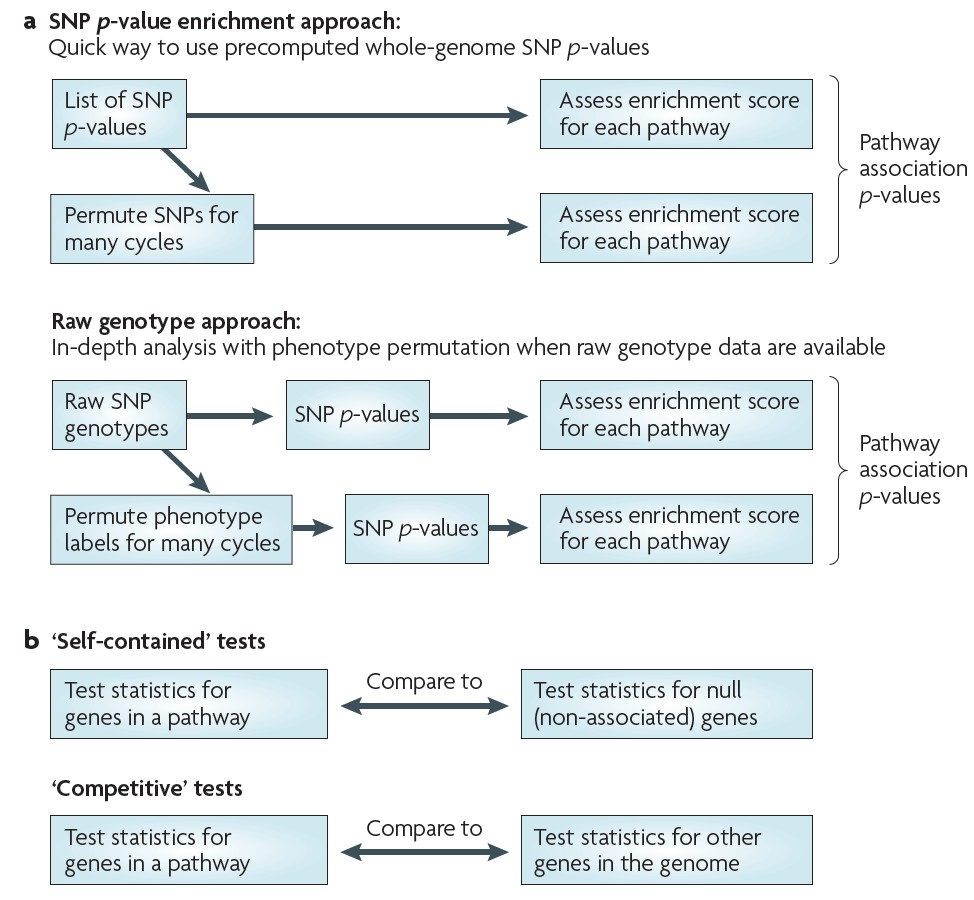
\includegraphics[scale=0.5]{pathwayTests_definition}
\label{fig: pathwayTests}
\caption{ \textbf{Types of pathway association tests in GWAS.} (a). Categorization based on data input type; (b). Categorization based on hypothesis testing. Figure is adopted from Wang et al 2010 \cite{Wang2010}. }
\end{figure}

There are already a few currently existed methods in testing pathway association which includes:  

pathway: grass [1], gseaSnp [4], plinkSet [3] and aligator [2]. Use

\newpage
%%%%%%%%%%%%%%%%%%%%%%%%%%%%%%%%%%%%%%%%%%%%%%%%%%%%%%%%%%%%
\section{Specific Aims and Hypotheses}\label{sec:aims}
%%%%%%%%%%%%%%%%%%%%%%%%%%%%%%%%%%%%%%%%%%%%%%%%%%%%%%%%%%%%

\begin{enumerate}
\item One

\item Two

\item ...
\end{enumerate}

\newpage
%%%%%%%%%%%%%%%%%%%%%%%%%%%%%%%%%%%%%%%%%%%%%%%%%%%%%%%%%%%%
\section{Data}\label{sec:data}
%%%%%%%%%%%%%%%%%%%%%%%%%%%%%%%%%%%%%%%%%%%%%%%%%%%%%%%%%%%%

\newpage
%%%%%%%%%%%%%%%%%%%%%%%%%%%%%%%%%%%%%%%%%%%%%%%%%%%%%%%%%%%%
\section{Methods}\label{sec:method}
%%%%%%%%%%%%%%%%%%%%%%%%%%%%%%%%%%%%%%%%%%%%%%%%%%%%%%%%%%%%


%%%%%%%%%%%%%%%%%%%%%%%%%%%%%%%%%%%%%%%%
\subsection{Subsection one}\label{sec:subsec1}
%%%%%%%%%%%%%%%%%%%%%%%%%%%%%%%%%%%%%%%%


%%%%%%%%%%%%%%%%%%%%%%%%%%%%%%%%%%%%%%%%
\subsubsection{Subsubsection one}\label{sec:subsub1-1}
%%%%%%%%%%%%%%%%%%%%%%%%%%%%%%%%%%%%%%%%%

%%%%%%%%%%%%%%%%%%%%%%%%%%%%%%%%%%%%%%%%%
\subsubsection{Subsubsection two}\label{sec:subsub1-2}
%%%%%%%%%%%%%%%%%%%%%%%%%%%%%%%%%%%%%%%%%


%%%%%%%%%%%%%%%%%%%%%%%%%%%%%%%%%%%%%%%%%
\subsection{Subsection two}\label{sec:subsec2}
%%%%%%%%%%%%%%%%%%%%%%%%%%%%%%%%%%%%%%%%%


%%%%%%%%%%%%%%%%%%%%%%%%%%%%%%%%%%%%%%%%%
\subsubsection{Subsubsection one}\label{sec:subsub2-1}
%%%%%%%%%%%%%%%%%%%%%%%%%%%%%%%%%%%%%%%%%



%%%%%%%%%%%%%%%%%%%%%%%%%%%%%%%%%%%%%%%%%
\subsubsection{Subsubsection two}\label{sec:subsub2-2}
%%%%%%%%%%%%%%%%%%%%%%%%%%%%%%%%%%%%%%%%%


\newpage
%%%%%%%%%%%%%%%%%%%%%%%%%%%%%%%%%%%%%%%%%
\section{Plan for Simulation Studies}\label{sec:simulation}
%%%%%%%%%%%%%%%%%%%%%%%%%%%%%%%%%%%%%%%%%



%%%%%%%%%%%%%%%%%%%%%%%%%%%%%%%%%%%%%%%%%
\subsection{Subsection one}\label{sec:subsimulation1}
%%%%%%%%%%%%%%%%%%%%%%%%%%%%%%%%%%%%%%%%%


%%%%%%%%%%%%%%%%%%%%%%%%%%%%%%%%%%%%%%%%%
\subsection{Subsection two}\label{sec:subsimulation2}
%%%%%%%%%%%%%%%%%%%%%%%%%%%%%%%%%%%%%%%%%

\begin{table}[H]
\begin{center}
\caption{Example table}
\begin{tabular}{cccccccccc}
\hline
&  & \multicolumn{2}{c}{\emph{A}} && \multicolumn{2}{c}{\emph{B}} & &\multicolumn{2}{c}{\emph{C}} \\
\cline{3-4}\cline{6-7}\cline{9-10}
\emph{par}& \emph{truth}& \emph{est}    & \emph{95\% CI} & & \emph{est.}    & \emph{95\% CI}  && \emph{est.} & \emph{95\% CI}\\
\hline
$\beta_1$ & 10 &   &( , )& &  & ( , )& &  &( , )\\
$\beta_2$ & 1 & &( ,  ) & &  & ( , )& &  &( , )\\
$\beta_3$ & -1 &  &( ,  ) & &  & ( , )& & &( , )\\
\hline
\end{tabular}
\end{center}
\end{table}




%%%%%%%%%%%%%%%%%%%%%%%%%%%%%%%%%%%%%%%%%
\subsubsection{Subsubsection one}\label{sec:subsimulation2-1}
%%%%%%%%%%%%%%%%%%%%%%%%%%%%%%%%%%%%%%%%%

\begin{figure}[H]
\centering

\includegraphics[scale=0.5]{SPH_2c_vert+below_lrg}
\label{fig: sample}
\caption{Sample figure.}
\end{figure}














%%%%%%%%%%%%%%%%%%%%%%%%%%%%%%%%%%%%%%%%%
\bibliographystyle{apalike}
\addcontentsline{toc}{section}{References}
\bibliography{proposal}
%%%%%%%%%%%%%%%%%%%%%%%%%%%%%%%%%%%%%%%%%

\end{document}
